\documentclass[a4paper,11pt,oneside]{article}
\usepackage[utf8]{inputenc}
\usepackage{setspace}
\usepackage{hyperref}
\usepackage{graphicx}
\graphicspath{ {images/}}
\usepackage[left=0.5in, right=2in, bottom=1in, top=0.5in]{geometry}
\pagenumbering{arabic}
\renewcommand{\familydefault}{\sfdefault}
\begin{document}

\noindent\LARGE{\textbf{ Hrushikesh Budhale}}  \\
\vspace{0ex}
\noindent\hrulefill
\normalsize


\begin{center}
\vspace{-3ex}
\begin{tabular}{l r}
Walchand College of Engineering,    & \hspace{2.5in} Contact: +91 9623928230\\
Sangli-416415,                      & \hspace{2.5in} e-mail id: \href{mailto:hruhnb@email.com}{hruhnb@email.com} \\
Maharashtra                         & \\
                                 & \hspace{2.5in} 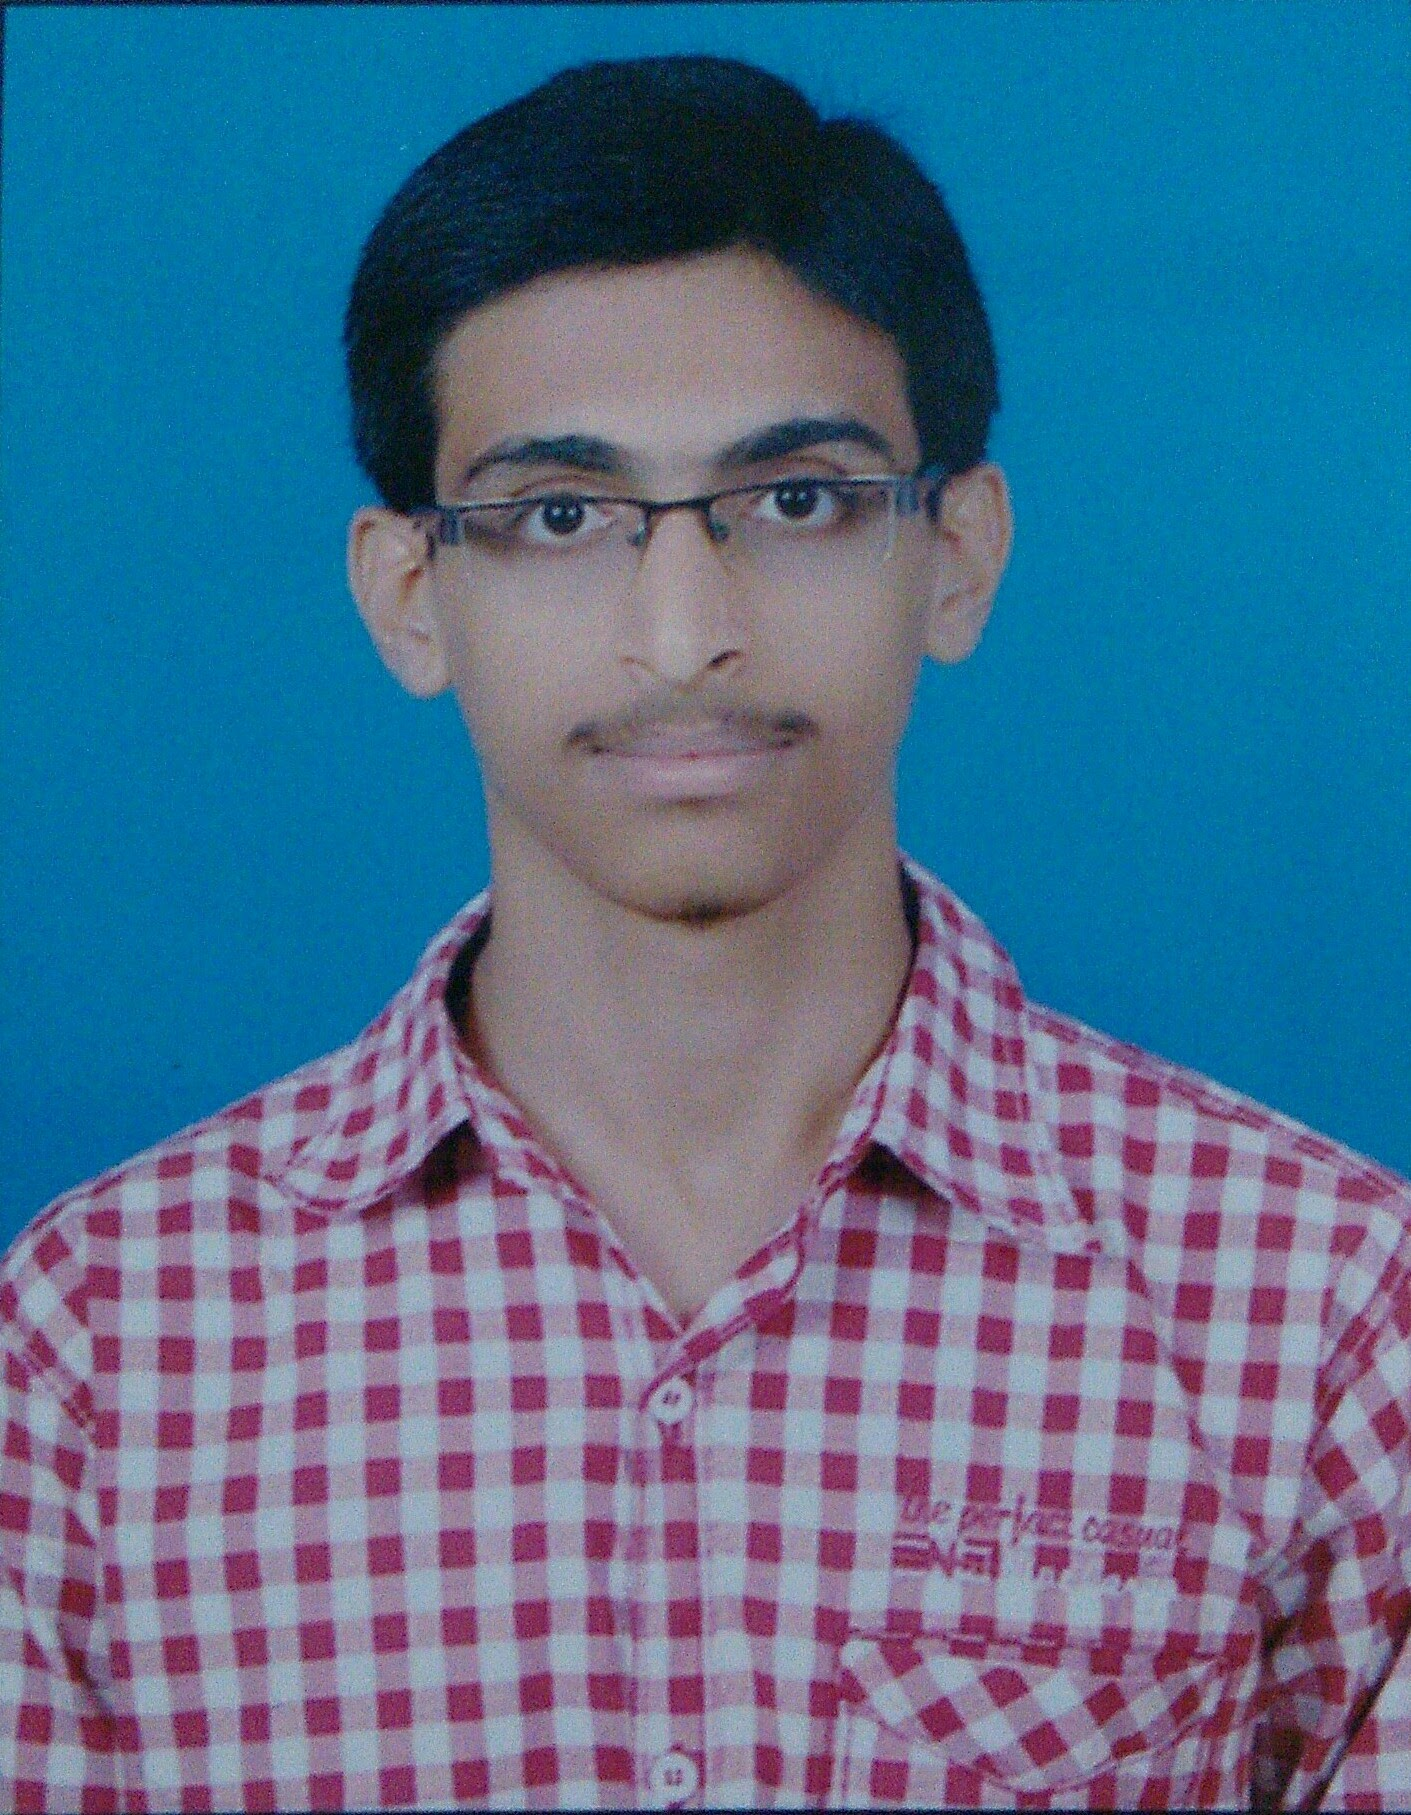
\includegraphics[scale=0.04]{id.jpg} \\
\end{tabular}
\end{center}

% \begin{flushright}
%     \includegraphics[scale=0.6]{Phillips} \\
% \end{flushright}

\noindent \begin{tabular}{@{} p{0.2\textwidth} p{\textwidth}}
 \textbf{\large{Objective}}
     & \large{Obtain an internship in  that will benefit from an advanced knowledge of} \\
     & \large{robotics and algorithmic programming skills.} \\ \\
     
 \textbf{\large{Education}}
     & \begin{tabular}[t]{ |l|c|l|l|l| }
            \hline
            \textbf{Degree} & \textbf{College/School} & \textbf{University} & \textbf{Passing} & \textbf{Pass} \\
            &  &  & \textbf{year} & \textbf{Percentage} \\
            \hline
            BTech & Walchand College of Engg., & Autonomous & 2018-19 & 8.01 \scriptsize{CGPA} \\ 
            & Sangli & & & \\ 
            \hline
            HSC & Shri Mhalsakant Vidyalaya,& Pune & 2014-15 & 82.86\%   \\ 
            & Chinchwad & & & \\ 
            \hline
            SSC & New English School, & Kolhapur & 2012-13 & 85.6\% \\ 
            & Satara & & & \\ 
            \hline
        
        \end{tabular}
        \vspace{2em} \\
        
 \textbf{\large{Projects}}    
     & \vspace{-1em}
       \begin{enumerate}
            \setlength\itemsep{0.1em}
            \item FPGA based development kit for microprocessor
            \item Weather dependent, remote programmable device for Precision Agriculture
            \item Remote controlled and voice activated Home Automation
            systems
            \item Water level controller for synchronization between overhead and underground tanks
        \end{enumerate} \\
 \textbf{\large{Training and}} & \\
 \textbf{\large{Internship}}
     & \vspace{-3em}
       \begin{itemize}
            \setlength\itemsep{0.1em}
            \item Online course ‘Intro to Python on Data Science’ on DATACAMP.
            \item Online course on ‘Machine Learning’ on COURSERA in MATLAB.
            \item Online course on ‘Machine Learning A-Z’ on UDEMY in python.
            \item Online course on ‘Getting started with Git’
            \item Open elective on ‘Internet of things’
        \end{itemize}  \\
 \textbf{\large{Research}} & \\
 \textbf{\large{Publication}} & \hspace{1em} --- ---  \\
\end{tabular}

\newpage
\noindent \begin{tabular}{@{} p{0.2\textwidth} p{\textwidth}}
 \textbf{\large{Technical skills }}
    & \vspace{-2em}
      \begin{itemize}
        \setlength\itemsep{0.1em}
        \item domain
        \item Digital Circuit Design
        \item Embedded Programming
        \item System Design
        \item Machine Learning
        \item Data Analytics
        \item Object oriented programming
    \end{itemize}\\ \\
    
 \textbf{\large{Soft Skills}}
    & \vspace{-2em}
      \begin{enumerate}
        \setlength\itemsep{0.1em}
        \item Time management
        \item Good team collaboration
        \item Adaptive to new concepts
        \item Creativity
      \end{enumerate} \\ \\
 
 \textbf{\large{Extra}} & \\
 \textbf{\large{Curricular}} & \\
 \textbf{\large{Activities}}
    & \vspace{-4em}
      \begin{itemize}
        \setlength\itemsep{0.1em}
        \item Served as Programmer and system design head in International Robotics competition `Robocon 2018'.
        \item Finalist of remote controlled boat buildig competition `AquaBot' in annual college event `vision 2016' arranged by Walchand College of Engg.
        \item Won award for `Best Interview' in `Impulse 2016'.
    \end{itemize}  \\ \\
 \textbf{\large{Co-Curricular}} & \\
 \textbf{\large{Activities}}
    & \vspace{-3em}
      \begin{enumerate}
        \setlength\itemsep{0.1em}
        \item Winner of  competition `E-Champ'.
        \item Winner of `Circuitron' a Digital Circuit Design Contest in an annual college event, organized by `Electronics Student Association' club of Walchand in 2016
        \item Served as team leader of Semifinalist Team in `E-Yantra 2016'.
        \item Runner-up of Digital Circuit Design Contest in annual college event in 2017
    \end{enumerate}
    \vspace{1em}\\
\end{tabular}

\noindent
\vspace{-1.5em}
\begin{tabular}{@{} p{0.25\textwidth} p{0.25\textwidth} p{\textwidth}}
 \textbf{\large{Personal}}           & Father's Name:  & Naresh M. Budhale \\
 \textbf{\large{Details}}            & Mother's Name:  & Poonam N. Budhale \\
                            & Sex:            & Male \\
                            & Date of Birth:  & 13-Aug-1998 \\
                            & Marital Status: & Unmarried \\ \\
\end{tabular}
\noindent \begin{tabular}{@{} p{0.25\textwidth} p{\textwidth}}
 \vspace{1em}
 \textbf{\large{Reference}} & \\ \\
 \textbf{\large{Declaration}}
    & I hereby declare that all the information provided in this resume is true \\
    & to the best of my knowledge and belief. \\ \\
 \textbf{\large{Date}} & 18-April-2018 \\
 
\end{tabular}


\clearpage

\end{document}